\documentclass{beamer}

\usetheme[headernav]{TACC} %%Drop the 'headernav' if you don't like
                           %%the stuff at the top of your slide

\usepackage{amsmath,amssymb,amsthm}
\usepackage{alltt}
\usepackage{graphicx}

\title{Lmod: What's New with TACC's Environment Module System}

\author{Robert McLay}
\institute{The Texas Advanced Computing Center}

\date{January, 22, 2018}  %% Use this if you want to fix the date in
                          %% stone rather than use \today

\newcommand{\bfnabla}{\mbox{\boldmath$\nabla$}}
\newcommand{\laplacian}[1]{\bfnabla^2 #1}
\newcommand{\grad}[1]{\bfnabla #1}
\newcommand{\tgrad}[1]{\bfnabla^T #1}
\newcommand{\dvg}[1]{\bfnabla \cdot #1}
\newcommand{\curl}[1]{\bfnabla \times #1}
\newcommand{\lap}[1]{\bfnabla^2 #1}

\begin{document}

\begin{frame}
  \titlepage
\end{frame}

\section{Introduction}

% page 2
\begin{frame}{Introduction}
  \begin{itemize}
    \item What is Lmod?
    \item Can Lmod help manage your site?
    \item Advanced Topics
    \item Where to go for help.
  \end{itemize}
\end{frame}

% page 3
\begin{frame}{Lmod's Big Ideas}
  \begin{itemize}
    \item A modern replacement for a tried and true concept.
    \item The guiding principal: ``Make life easier w/o getting in
      the way.''
    \item Reads both TCL and Lua modulefiles including Cray Modulefiles.
  \end{itemize}
\end{frame}

% page 4
\begin{frame}{Fundamental Issues}
  \begin{itemize}
    \item Software Packages are created and updated all the time.
    \item Some Users need new versions for new features and bug fixes.
    \item Other Users need older versions for stability and continuity.
    \item No system can support all versions of all packages.
    \item User programs using pre-built C++ \& Fortran libraries must link with the same compiler.
    \item Similarly, MPI Applications must build and link with same
      MPI/Compiler pairing when using pre-built MPI libraries.
  \end{itemize}
\end{frame}

% page 5
\begin{frame}[fragile]
    \frametitle{Example of Lmod: Environment Modules (I)}
    {\tiny
\begin{semiverbatim}
{\color{blue}\$ module list}
Currently Loaded Modules:
  1) StdEnv  2) gcc/4.5  3) mpich2/1.4  4) petsc/3.1
{\color{blue}\$ module unload gcc}
Inactive Modules:
  1) mpich2  2) petsc
{\color{blue}\$ module list}
Currently Loaded Modules:
  1) StdEnv
Inactive Modules:
  1) mpich2  2) petsc
{\color{blue}\$ module load intel}
Activating Modules:
  1) mpich2  2) petsc
{\color{blue}\$ module swap intel gcc}
Due to MODULEPATH changes the follow modules have been reloaded:
  1) mpich2  2) petsc
{\color{blue}\$ module load gcc}
Due to MODULEPATH changes the follow modules have been reloaded:
  1) mpich2  2) petsc
\end{semiverbatim}
    }
\end{frame}

% page 6
\begin{frame}[fragile]
    \frametitle{Example of Lmod: Environment Modules (II)}
    {\tiny
\begin{semiverbatim}
\$ {\color{blue} module avail}
------------------ /opt/apps/modulefiles/MPI/intel/12.0/mpich2/1.4 ------------------
  petsc/3.1 (D)    petsc/3.1-debug    pmetis/4.0    tau/2.20.3

------------------- /opt/apps/modulefiles/Compiler/intel/12.0 -----------------------
  boost/1.45.0        gotoblas2/1.13      openmpi/1.4.3
  boost/1.46.0        mpich2/1.3.2        openmpi/1.5.1
  boost/1.46.1 (D)    mpich2/1.4    (D)   openmpi/1.5.3   (D)

-------------------------- /opt/apps/modulefiles/Core -------------------------------
  StdEnv               intel/11.1         papi/4.1.4
  admin/admin-1.0      intel/12.0  (D)    scite/2.28
  ddt/ddt              lmod/lmod          tex/2010
  dmalloc/dmalloc      local/local (D)    unix/unix    (D)
  fdepend/1.2          mkl/mkl            visit/visit
  gcc/4.4              noweb/2.11b
  gcc/4.5        (D)
\end{semiverbatim}
    }
\end{frame}

% page 7
\begin{frame}{Why does Lmod work at all?}
  \begin{itemize}
    \item The environment is inherited from the parent process
    \item Changes in a child process \emph{DOES NOT} affect the
      parent's environment
    \item So how could Lmod work at all?
  \end{itemize}
\end{frame}

% page 8
\begin{frame}{The trick is:}
  \begin{itemize}
    \item The \texttt{lmod} program generates text.
    \item The module command eval's that text.
    \item \texttt{module() \{eval \$(\$LMOD\_CMD bash "\$@";)\}}
    \item \texttt{stdout} is evaluated
    \item \texttt{stderr} passes through
  \end{itemize}
\end{frame}

% page 9
\begin{frame}{Why You Might Want To Use Lmod}
  \begin{itemize}
    \item Same \texttt{module} command as in Tmod
    \item Active Development;  Frequent Releases; Bug fixes.
    \item Vibrant Community
    \item It is used from Norway to Isreal to New Zealand from Stanford to MIT to NASA
    \item Enjoy many capabilities w/o changing a single module file
    \item Debian and Fedora packages available
    \item Many more advantages when you're ready
    \item It is what we use every day!
  \end{itemize}
\end{frame}


% page 10
\begin{frame}{Features}
  \begin{itemize}
    \item Reads for TCL and Lua modulefiles
    \item One name rule.
    \item Support Software Hierarchy (single parent only!)
    \item Spider Cache: fast \texttt{\color{blue} \$ module avail}
    \item Properties (gpu, mic)
    \item Semantic Versioning:  5.6 is older than 5.10
    \item family(``compiler'') family(``mpi'') support
    \item Optional Tracking: What modules are used?
    \item Many other features: ml, collections, hooks, Env Vars, ...
  \end{itemize}
\end{frame}

% page 11
\begin{frame}{History of Support for Module Names}
  \begin{itemize}
    \item Originally only \emph{name/version (N/V)}:  gcc/4.8.1
    \item Lmod 5+ \emph{cat/name/version (C/N/V)}:  compiler/gcc/4.8.1
    \item Lmod 7+ \emph{name/version/version (N/V/V)}: intel/impi/64/18.0.1
  \end{itemize}
\end{frame}

% page 12
\begin{frame}{New with Lmod 7: N/V/V}
  \begin{itemize}
    \item Support for \emph{name/v1/v2}:  fftw/64/3.3.4
    \item MODULERC Support:
      \begin{itemize}
        \item Set Defaults under Site and/or User
        \item Hide any installed module
      \end{itemize}
    \item Major refactoring of Lmod 
      \begin{itemize}
        \item support N/V/V
        \item Code Cleanup
        \item Better Spider Cache handling
      \end{itemize}
  \end{itemize}
\end{frame}

% page 13
\begin{frame}{Setting Defaults}
  \begin{itemize}
    \item System MODULERC file: \texttt{/path/to/lmod/etc/rc}
    \item \texttt{\$MODULERC} points to a file.
    \item User \texttt{\textasciitilde/.modulerc}
    \item Can set defaults User, System, Files
    \item Examples: account for web services
  \end{itemize}
\end{frame}

% page 14
\begin{frame}{Hiding Modules}
  \begin{itemize}
    \item System MODULERC file: \texttt{/path/to/lmod/etc/rc}
    \item User \texttt{\textasciitilde/.modulerc}
    \item \texttt{\color{blue}hide-version foo/1.2.3}
    \item Hidden from avail, spider and keyword
    \item Hidden modules can be loaded
    \item Sites: deprecation, experimental
    \item show hidden: \texttt{module --show-hidden avail}
  \end{itemize}
\end{frame}


% page 15
\begin{frame}{Recent Improvements}
  \begin{itemize}
    \item New module function: \texttt{depends\_on()}
    \item Reference counting on PATH like variables
    \item French, German, Spanish translations for Lmod messages.
    \item Admin list (AKA Nag List) supports Lua Regex for matching
    \item Improved Settarg (more on this later?)
  \end{itemize}
\end{frame}

% page 16
\begin{frame}{\texttt{depends\_on()}}
  \begin{itemize}
    \item Modules X and Y depends on Module A
    \item ml purge; ml X; ml unload X;      $\Rightarrow$ unload A
    \item ml purge; ml X Y; ml unload X;    $\Rightarrow$ keep A
    \item ml purge; ml X Y; ml unload X Y ; $\Rightarrow$ unload A
    \item ml purge; ml A X Y; ml unload X Y ; $\Rightarrow$ keep A
  \end{itemize}
\end{frame}

% page 17
\begin{frame}{Reference Counting for PATH like variables}
  \begin{itemize}
    \item AKA: the /usr/local/bin problem
    \item Old:
      \begin{itemize}
        \item Default path has /usr/local/bin
        \item Module A also has /usr/local/bin
        \item Unloading module A removes /usr/local/bin from path
      \end{itemize}
    \item New: With Ref. Count the problem is fixed.
  \end{itemize}
\end{frame}

% page 18
\begin{frame}{MODULEPATH ref counting}
  \begin{itemize}
    \item A user has requested the MODULEPATH have ref-counting
    \item \texttt{ml unuse /path/to/modules} would always remove
      directory from MODULEPATH
    \item This is now implemented.
  \end{itemize}
\end{frame}

% page 19
\begin{frame}{Future Work (I): Module Export}
  \begin{itemize}
    \item Module Collections are for individuals.
    \item They are not meant to be shared between users
    \item To share I plan to add ``module export''
  \end{itemize}
\end{frame}


% page 20
\begin{frame}[fragile]
    \frametitle{Module Export}
    {\tiny
\begin{semiverbatim}
    \$ module export <collection> > export.txt
    \$ cat export.txt

    module purge
    clearMT
    export MODULEPATH=/path1:/path2
    
    module collection_load X Y Z
    module --ref_count 2 depend_on A
\end{semiverbatim}
    }
\end{frame}

% page 21
\begin{frame}[fragile]
    \frametitle{Lmod Doc usage}
    \center{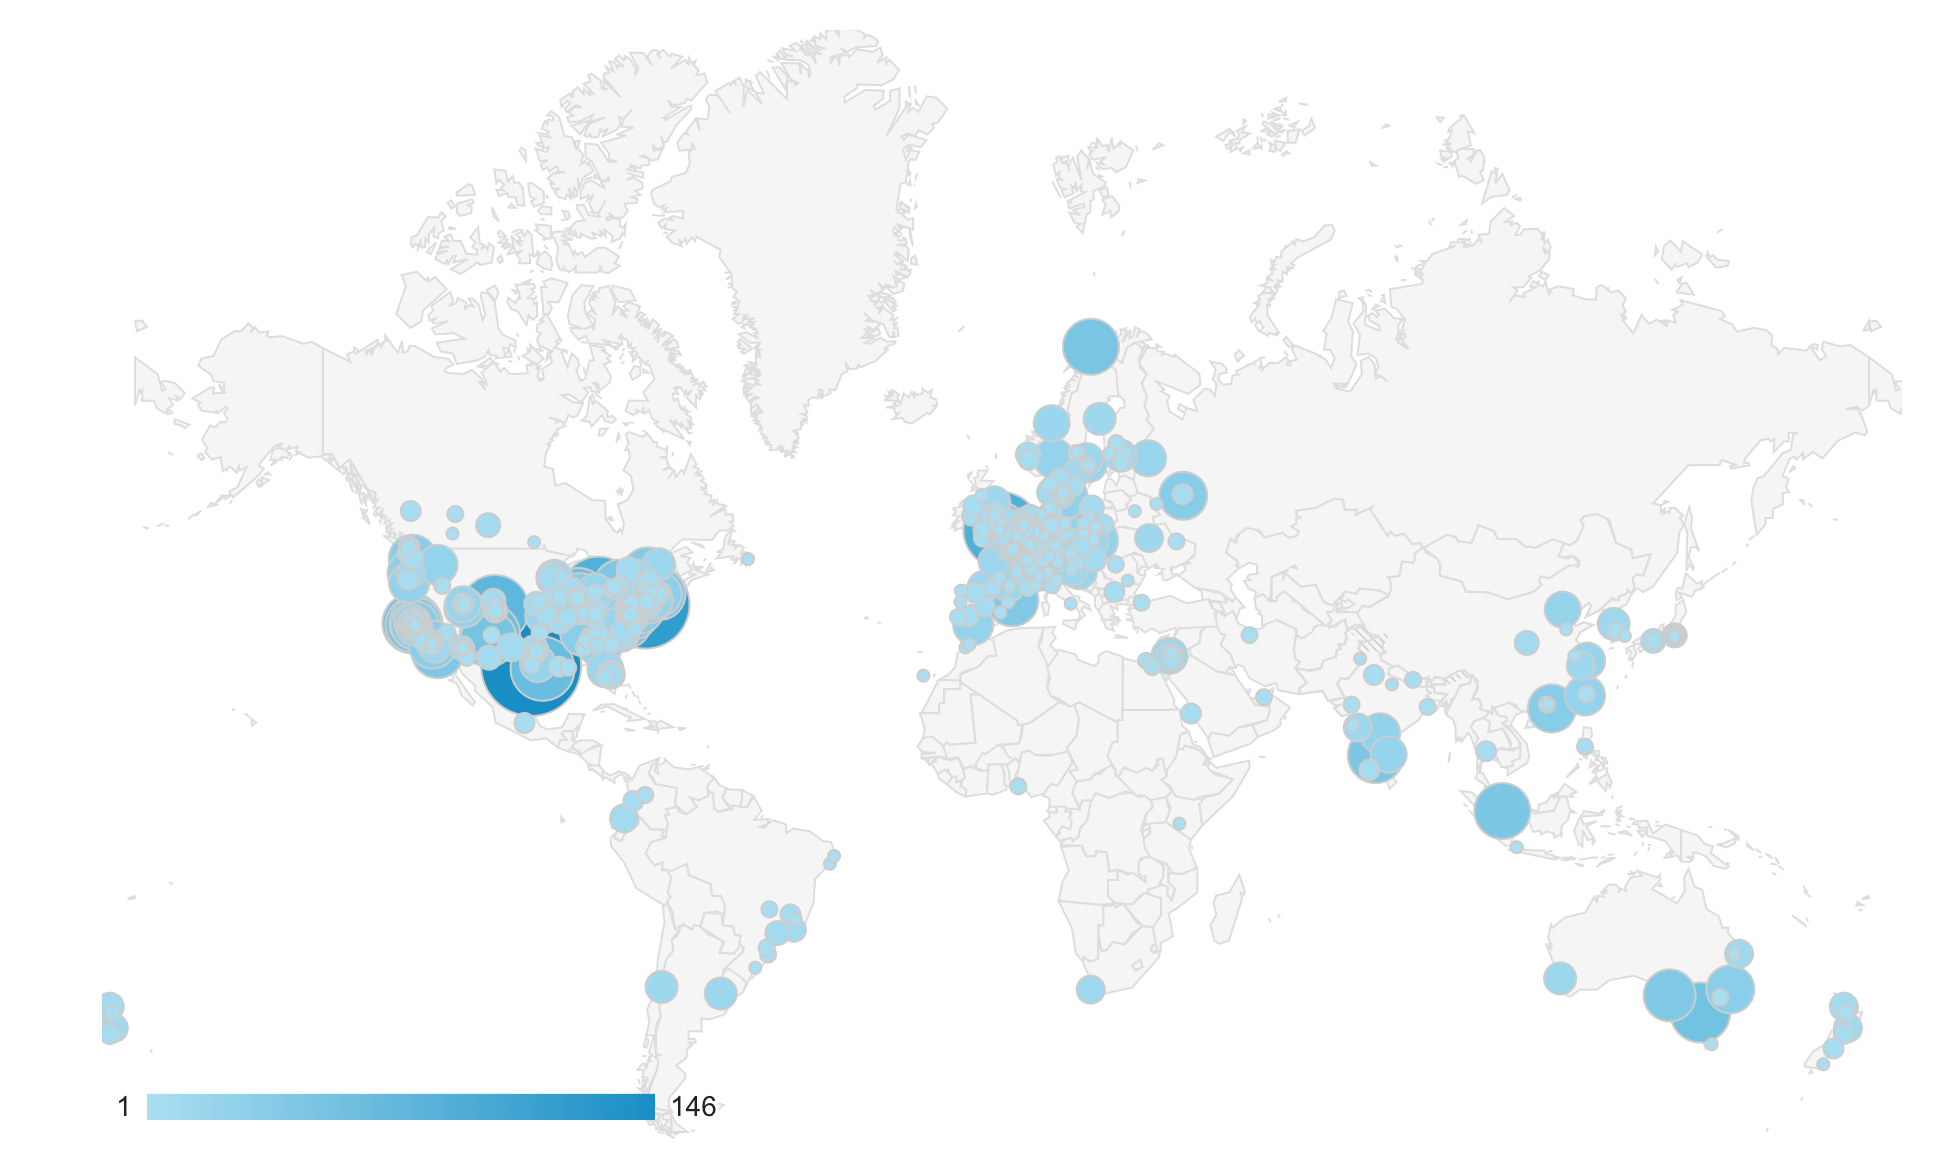
\includegraphics[width=.9\textwidth]{Lmod_docs_usage}}
\end{frame}


% page 22
\begin{frame}{Can tools like Lmod improve the user experience?}
  \begin{itemize}
    \item Sites provide packages: applications and libraries
    \item Users can pick which packages and version to suit their needs
    \item But what we are really after is to cut down on tickets!
    \item Or simply make your resources easier for your users
  \end{itemize}
\end{frame}

% page 23
\begin{frame}{Lmod examples}
  \begin{itemize}
    \item Lmod was first released in 2009
    \item It is the only module system used at TACC since 2010
    \item The following are some examples of how Lmod can help
  \end{itemize}
\end{frame}

% page 24
\begin{frame}{Can Lmod help with the /usr/local/bin problem?}
  \begin{itemize}
    \item Suppose your startup files put /usr/local/bin in PATH
    \item And suppose module BAR also adds /usr/local/bin to PATH
    \item Currently Loading then unloading BAR will remove
      /usr/local/bin from PATH. 
    \item Site can configure Lmod to support duplicate paths
    \item Lmod now supports reference counting!
  \end{itemize}
\end{frame}

% page 25
\begin{frame}{Can Lmod prevent users from mixing modules they shouldn't?}
  \begin{itemize}
      \item Same Name modules:
      \begin{itemize}
        \item Things can get confusing when users load two gcc modules
        \item Normally, Lmod will unload old gcc, then load new gcc
        \item Optionally, sites can auto-conflict with themselves.
      \end{itemize}
    \item Loading two compilers or MPI Stack:
      \begin{itemize}
        \item It is a rare user who needs to load two different
          compilers or two MPI stacks
        \item GCC and Intel are a special case
        \item Sites can add family("compiler") to compiler modules
        \item This will autoswap one compiler for another!
        \item Similarly for MPI modules.
      \end{itemize}
  \end{itemize}
\end{frame}

% page 26
\begin{frame}{How to manage software: New or Old}
  \begin{itemize}
    \item How can you test new/experimental software?
    \item Suppose your site keeps SW for the life of machine?
    \item How do you encourage usage of newer SW w/o breaking old job
      scripts?
    \item Lmod now supports hiding regular modules from avail and
      spider.
    \item Hidden modules can still be loaded.
    \item Modules can be explicitly marked as hidden
    \item Or you can use the isVisible hook
    \item Both sites and users can hide modules
  \end{itemize}
\end{frame}

% page 27
\begin{frame}{Can Lmod help with deprecating packages?}
  \begin{itemize}
    \item Suppose your site keeps a limited number of versions (say 3
      or less)
    \item How to you decide which package to keep or remove?
    \item Lmod support optional tracking of what packages are loaded
      by whom.
    \item You can send targeted email to those users about
      deprecation based on tracking.
    \item Independent of tracking: nag messaging
    \item Do not need to change modulefile!
    \item Users get a message when they load a deprecated module. 
  \end{itemize}
\end{frame}

% page 28
\begin{frame}{Can Lmod help a site that does not want default modules?}
  \begin{itemize}
    \item Suppose your site produces weather forecasts or processes
      satellite images.
    \item No one set of compilers etc will satify your needs.
    \item Site can set LMOD\_EXACT\_MATCH$=$yes $\Rightarrow$ There are no defaults
    \item Users \emph{MUST} specify name and version!
  \end{itemize}
\end{frame}

% page 29
\begin{frame}{Can users have their own default list of modules?}
  \begin{itemize}
    \item It is common to provide a default list of modules
    \item However some users will want their own modules at startup
    \item Users can add module commands to \textasciitilde/.bashrc etc
    \item But this is tricky to get right.
    \item Lmod supports default module collections
    \item In fact, users can have as many named collections as they like.
  \end{itemize}
\end{frame}


% page 30
\begin{frame}{Can Lmod deal with shared home filesystem?}
  \begin{itemize}
    \item Suppose your site shares the home filesystem across two or
      more clusters
    \item These clusters have different modules.
    \item Site can set \$LMOD\_SYSTEM\_NAME uniquely on each cluster
    \item This way user's collection (and personal caches) will be
      unique
  \end{itemize}
\end{frame}

% page 31
\begin{frame}{Can users easily grep the output from Lmod?}
  \begin{itemize}
    \item Lmod sends messages to \texttt{stderr} by default
    \item Lmod can redirect the output to \texttt{stdout} by setting
      \$LMOD\_REDIRECT=yes
    \item This works for bash, zsh
    \item It doesn't work for csh/tcsh due to the way eval works there
    \item Setting \$LMOD\_REDIRECT=yes means you lose the pager
    \item I do this instead: \$ module --raw --redirect show impi |
      grep tmi
  \end{itemize}
\end{frame}

% page 32
\begin{frame}{Can Lmod work with Localization and Site Messages?}
  \begin{itemize}
    \item Starting Lmod 7.1+ Lmod provides the possibility of Language
      Translations: ES, FR, DE, and ZH
    \item Sites can also provide tailored message to suit their needs
  \end{itemize}
\end{frame}

% page 33
\begin{frame}{Can Lmod help with software web pages?}
  \begin{itemize}
    \item Many sites want to provide web pages that list the SW
      they provide.
    \item Lmod provides a tool to generate a JSON or XML list of all
      system modules.
    \item You'll have to write something to ingest the JSON or XML
  \end{itemize}
\end{frame}

% page 34
\begin{frame}{Can Lmod help with compiler and/or MPI/compiler
      dependent modules?}
  \begin{itemize}
    \item Sites can chose a Flat or Hierarchical Naming Scheme
    \item PETSc: A parallel iterative solver package:
      \begin{itemize}
        \item Compilers: GCC 6.3, Intel 17.0
        \item MPI Implementations: MVAPICH2 2.1, IMPI 17.0
        \item MPI Solver package: PETSc 4.1
        \item 4 versions of PETSc: 2 Compilers $\times$ 2 MPI
      \end{itemize}

    \item Flat layout for PETSc
      \begin{enumerate}
        \item \texttt{PETSc/4.1-mvapich2-2.1-gcc-6.3}
        \item \texttt{PETSc/4.1-mvapich2-2.1-intel-17.0}
        \item \texttt{PETSc/4.1-impi-17.0-gcc-6.3}
        \item \texttt{PETSc/4.1-impi-17.0-intel-17.0}
      \end{enumerate}
  \end{itemize}
\end{frame}

% page 35
\begin{frame}{Problems w/ Flat naming scheme}
  \begin{itemize}
    \item Users have to load modules:
      \begin{itemize}
        \item ``intel/17.0''
        \item ``mvapich2/2.1-intel-17.0''
        \item ``PETSc/4.1-mvapich2-2.1-intel-17.0''
        \item Changing compilers means unloading all three modules
        \item Reloading new compiler, MPI, PETSc modules.
        \item Not loading correct modules $\Rightarrow$ Mysterious Failures!
        \item Onus of package compatibility on users!
        \item Or extremely complicated modulefiles!
        \item Tools like EasyBuild or Spack can help here.
      \end{itemize}
  \end{itemize}
\end{frame}

%page 36
\begin{frame}{Hierarchical Naming Schemes}
  \begin{itemize}
    \item Store modules under one tree: \texttt{/opt/apps/modulefiles}
    \item One strategy is to use sub-directories:
      \begin{itemize}
        \item Core: Regular packages: apps, compilers, git
        \item Compiler: Packages that depend on compiler: boost, MPI
        \item MPI: Packages that depend on MPI/Compiler: PETSc, FFTW3
      \end{itemize}
  \end{itemize}
\end{frame}

%page 37
\begin{frame}{Loading the correct module}
  \begin{itemize}
    \item User loads ``\texttt{intel/17.0}'' module
    \item Can only see/load compiler dependent packages that are built with
      intel 17.0 compiler.
    \item Can not see/load package built with other versions or other compilers.
    \item Similar loading ``\texttt{mvapich2/2.1}'' module.
    \item Users can only load package that are built w/ intel 17.0 and
      mvapich2 2.1 and no others.
  \end{itemize}
\end{frame}

% page 38
\begin{frame}{Lmod works with both flat or hierarchy layouts}
  \begin{itemize}
    \item Sites can chose either kind of layout.  
    \item Lmod offers many advantages with either layout
    \item An Lmod site sys-admin transitioned his users by leaving the
      old system active
    \item A new hierarchy was available where all new SW was installed.
    \item Users can transition if/when they like.
  \end{itemize}
\end{frame}

%page 39
\begin{frame}{Bash Issues}
  \begin{itemize}
    \item Bash Startup is typically ``broken'' for non-login interactive shells
    \item Redhat, Centos, MacOS typically don't source /etc/bashrc on interactive shells
    \item MPI jobs start an interactive shell.
  \end{itemize}
\end{frame}

%page 40
\begin{frame}{Bash Issues (II)}
  \begin{itemize}
    \item Want module command to work in all shells.
    \item Want stacksize unlimited for MPI jobs
    \item We patched bash to force it to source /etc/tacc/bashrc
  \end{itemize}
\end{frame}

%page 41
\begin{frame}{Bash Repair Choices}
  \begin{itemize}
    \item Switch users to Z shell?
    \item patch bash (see Lmod docs)
    \item Expect all users to source /etc/bashrc in \textasciitilde/.bashrc
    \item Expect all users to start jobs with \#!/bin/bash -l
  \end{itemize}
\end{frame}

%page 42
\begin{frame}{Debugging Lmod}
  \begin{itemize}
    \item \texttt{module --config} : reports Lmod configuration
    \item \texttt{module -D load foo $>$ load.log}
  \end{itemize}
\end{frame}

%page 43
\begin{frame}{Tracing Lmod}
  \begin{itemize}
    \item A new feature of Lmod 7.4.4+
    \item module -T ...
    \item export LMOD\_TRACING=yes
    \item Can trace loads and how restores work.
  \end{itemize}
\end{frame}

%page 44
\begin{frame}{Conclusions: Lmod 7+}
  \begin{itemize}
    \item Latest version: https://github.com:TACC/Lmod.git
    \item Stable version: http://lmod.sf.net
    \item Documentation:  http://lmod.readthedocs.org
  \end{itemize}
\end{frame}


\end{document}
